%\hspace*{0.82cm}\\[0.5cm]
\chapter{Literature Survey}
\section{Android}
\hspace*{0.82cm}Google usually refers to the Android OS as a \textbf{software stack}. Each layer of 
the stack groups together several programs that support specific operating system functions. These
layers are illustrated in Figure 2.1.\\[0.5cm]
\hspace*{0.82cm}The base of the stack is the \textbf{kernel}. Google used the Linux version 2.6 OS to build
Android's kernel, which includes Android's memory management programs, security settings,
power management software and several hardware drivers. The next level of software
includes Android's \textbf{libraries}. Libraries are a set of instructions that tell the device how to
handle different kinds of data. Android runtime layer includes a set of core \textbf{Java} libraries --
Android application programmers build their apps using the Java programming language. It
also includes the Dalvik Virtual Machine. The next layer is the \textbf{application framework}. This
includes the programs that manage the phone's basic functions like resource allocation,
telephone applications, switching between processes or programs and keeping track of the
phone's physical location. Application developers have full access to Android's application
framework.
\begin{enumerate}[a. ]
 \item Application Framework is used to write applications for Android. Unlike other
embedded mobile environments, Android applications are all equal, for instance,
applications which come with the phone are no different than those that any developer
writes. The framework is supported by numerous open source libraries such as
openssl, sqlite and libc. It is also supported by the Android core libraries. From the
point of security, the framework is based on UNIX file system permissions that assure
applications have only those abilities that mobile phone owner gave them at install
time.
 \item Dalvik virtual machine is extremely low-memory based virtual machine, which was
designed especially for Android to run on embedded systems and work well in low
power situations. It is also tuned to the CPU attributes. The Dalvik VM creates a
special file format \texttt{(.DEX)} that is created through build time post processing.
Conversion between Java classes and \texttt{.DEX} format is done by included “dx” tool.
 \item Integrated browser, WebKit is chosen as an open source web browser. Google added
a two pass layout and frame flattening. Two pass layout loads a page without waiting 
for blocking elements, such as external CSS or external JavaScript and after a while
renders again with all resources downloaded to the device. Frame flattening converts
founded frames into single one and loads into the browser. These features increase
speed and usability browsing the internet via mobile phone.
 \item Optimized graphics – as Android has 2D graphics library and 3D graphics based on
OpenGL ES 1.0, great applications like Google Earth and spectacular games like
Second Life are seen, which come on Linux version. At this moment, the shooting
legendary 3D game Doom was presented using Android on the mobile phone.
\item SQLite is used, which is extremely small (~500kb) relational database management
system that is integrated in Android. It is based on function calls and single file,
where all definitions, tables and data are stored. This simple design is more than
suitable for a platform such as Android.
\end{enumerate}
\hspace*{0.82cm}There are a number of hardware dependent features, for instance, a huge media and
connections support, GPS, improved support for Camera and simply GSM telephony. A great
work was done for the developers to start work with Android using device emulator, tools for
debugging and plugin for Eclipse IDE.

\begin{figure}[H]
  \centering
    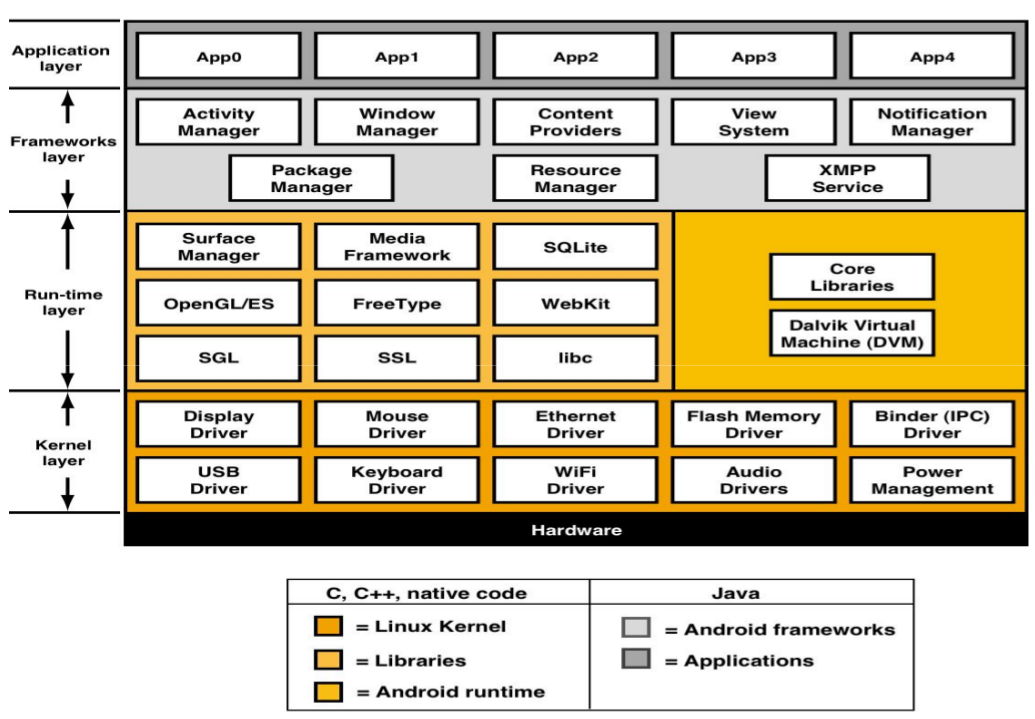
\includegraphics[scale=0.45]{project/images/system-architecture}
  \caption{\textbf{System Architecture}}
\end{figure}

Android Architecture is based on Linux 2.6 kernel. It helps to manage security,
memory management, process management, network stack and other important issues.
Therefore, the user should bring Linux in his mobile device as the main operating system and
install all the drivers required in order to run it. Android provides the support for the
Qualcomm MSM7K chipset family. For instance, the current kernel tree supports Qualcomm
MSM 7200A chipsets with stable version Qualcomm MSM 7200, which includes major
features:
\begin{itemize}
 \item WCDMA/HSUPA and EGPRS network support
 \item Bluetooth 1.2 and Wi-Fi support
 \item Digital audio support for mp3 and other formats
 \item Support for Linux and other third-party operating systems
 \item Java hardware acceleration and support for Java applications
 \item Qcamera up to 6.0 megapixels
 \item gpsOne – solution for GPS
 \item and lots of other features.
\end{itemize}

\section{Android and Synchronization}
\hspace*{0.82cm}The fast paced technology has changed the world as well as its habitants. In Today’s
global village there is no need to grab the telephone receiver and dial a specific number to
transmit voice through cables merely to hear the voice of a beloved. Now each of us carries
our own handsets with a built-in phonebook and text messages. The facilities like Wi-Fi and
internet have further improved the standard of communications by cutting down expenditure
and increasing availability.\\[0.5cm]
\hspace*{0.82cm}Regardless of the location, the world of web can be accessed through handsets,
laptops and tablet PCs. These modern times give us the necessity to maintain highly
important data on these portable devices so that we can access them on the go. But carrying
around this important data brings with it the risk of data getting corrupted due to hardware
failure, natural elements like rain spoiling our gadgets or the devices hard drive failing due to
shocks during transit.\\[0.5cm]
\hspace*{0.82cm}Hence to be safe and sure against such incidents it has become extremely to back up
our data after short intervals. Currently, the features of synchronization are available in
android devices, but they have a catch. These services are provided by third-party software
managers for e.g., Google.\\[0.5cm]
\hspace*{0.82cm}To back up our data, the data must be first synchronized with our Google account.
This means sending our extremely important data to the Google Clouds. This directly affects
the security and privacy aspects of the user. The data being stored on the Google cloud may
not be guarded securely. It is not guaranteed data will be safe and not private.\\[0.5cm]
\hspace*{0.82cm}Hence to overcome these restrictions, we have proposed a system where each user can
synchronize his/her phone with his/her own private server running anywhere. This will
ensure that all the data remains on our own private devices and no third-party can get hold of
this data.\\[0.5cm]
\hspace*{0.82cm}This means after synchronizing our private data like emails, SMS messages, contacts,
calendar entries, notes, documents, folders etc., all the data remains on the users server itself.
The server can be a Desktop Computer or a laptop connected to the internet. Also the android
devices can be synchronized in an offline manner.\\[0.5cm]
\hspace*{0.82cm}Offline sync can be done using Wi-Fi, Bluetooth or USB cable. Online sync will be
done via a secure connection over the internet. Using this product, the android user can be
ensured all their data remains on their own premises, no unnecessary sharing will be done to
third-parties, multiple copies of data can be maintained over multiple servers for additional
backup, if necessary.\\[0.3cm]

\begin{figure}[H]
  \centering
    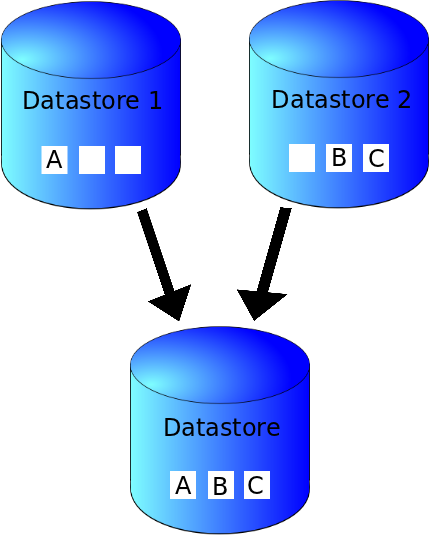
\includegraphics[height= 10cm, width=9cm]{project/images/data-sync}
  \caption{\textbf{Data Synchronization}}
\end{figure}